\documentclass[conference]{IEEEtran}
\IEEEoverridecommandlockouts
\usepackage{cite}
\usepackage{amsmath,amssymb}
\usepackage{booktabs}
\usepackage{graphicx}
\usepackage[table]{xcolor}
\usepackage{url}
\usepackage[hidelinks,pdfauthor={},pdfcreator={},pdfproducer={}]{hyperref}
\newif\ifanonymous
\anonymoustrue   % set \anonymousfalse for the camera-ready / single-blind version
\newif\ifappendix
\appendixtrue    % set \appendixfalse if the venue counts appendices toward the page limit
\newcommand{\confirm}[1]{\textcolor{red}{[#1]}}
\newcommand{\artifact}{\ifanonymous\url{https://anonymous.4open.science/r/XXXXXXXX}\else\confirm{public repository URL}\fi}

\begin{document}

\title{HoNE: Hold-out and Natural-Novelty Evaluation of Learned NIDS for Zero-Day Detection}

\ifanonymous
\author{\IEEEauthorblockN{Anonymous Author(s)}\IEEEauthorblockA{Submission under double-blind review}}
\else
\author{\IEEEauthorblockN{Gracious Mwamughunda, Guohao Sun\IEEEauthorrefmark{1}, Hafsa Aslam}
\IEEEauthorblockA{Donghua University, Shanghai, China\\
Email: 324078@mail.dhu.edu.cn, ghsun@dhu.edu.cn, 324091@mail.dhu.edu.cn\\
\IEEEauthorrefmark{1}Corresponding author}}
\fi
\maketitle

\begin{abstract}
Operators deploy learned network intrusion detection systems (NIDS) to catch attacks that did not exist at training time. Zero-day claims are typically supported by leave-one-attack-class-out (LOACO) evaluation, in which one attack class is withheld from a randomly split benchmark and the detector is scored once by AUC. Whether this evidence predicts how a detector behaves when a new attack arrives later in time has not been tested. We introduce HoNE (Hold-out and Natural-novelty Evaluation), a pre-registered, leakage-controlled benchmark that scores the same detectors, data and seeds under LOACO and under natural novelty, where attack classes first appear after the training period, including four rolling cut-points. We evaluate four NetFlow-v3 datasets and Lycos2017 with 12 detectors on a recurrent backbone, replicated on a GRU, over five seeds and 45 class--cut units. Five findings emerge. Temporal LOACO is infeasible on all three day-scheduled datasets. The winning detector family changes with protocol, dataset and cut-point. Natural novelty raises seed variability by up to 17$\times$. Max-softmax and energy fall below chance on both backbones. AUCs of 0.53--0.75 mean at most 18\% of novel attacks caught at 1\% false-positive rate. HoNE turns these findings into eight checks operators can require before trusting a zero-day claim.
\end{abstract}

\begin{IEEEkeywords}
network intrusion detection, network security management, zero-day attacks, evaluation methodology, NetFlow
\end{IEEEkeywords}

\section{Introduction}
\label{sec:intro}
Network operators increasingly rely on machine-learning network intrusion detection systems (NIDS) because signature rules cannot cover attacks that did not exist when the rules were written. The value of such a detector lies almost entirely in its \emph{zero-day} behaviour: an attack it has already seen could equally be caught by a signature. Before a learned NIDS is trusted in production, therefore, someone must decide whether its zero-day claim is credible, and that decision usually rests on evidence supplied by the detector's developers.

The stakes of that decision are operational. A detector whose zero-day performance has been overstated misses the attacks it was bought to catch, while one whose performance varies from training run to training run gives the security team no stable basis for setting alert thresholds or staffing triage. Both failures surface only after deployment, when the cost of discovering them is highest. The quality of pre-deployment evidence is therefore a network-management question, not only a machine-learning one.

The evidence in current use has a remarkably uniform shape, and each of its parts rests on an assumption that is rarely tested. Zero-day ability is usually measured by withholding one or a few attack classes from training on a benchmark split at random, so that the detector must flag them at test time~\cite{wilkie2026}; we call the one-class-at-a-time form \emph{leave-one-attack-class-out} (LOACO). Random splits let near-identical flows and whole attack episodes appear in both training and test sets~\cite{arp2022}, and LOACO keeps the benign traffic of the test period in training, so the held-out class is the only thing that changes. Results usually come from one training run, and novelty is often scored with confidence measures such as maximum softmax probability~\cite{hendrycks2017} or energy~\cite{liu2020energy}, which were designed for multi-class image recognition. The security-ML literature has long warned that such benchmark scores overstate field performance~\cite{sommer2010,apruzzese2023sok}.

What has not been tested is whether LOACO evidence predicts the situation an operator actually faces: a new attack class that arrives \emph{later in time}, alongside drifting benign traffic, which we call \emph{natural temporal novelty}. Answering this requires scoring the same detectors, on the same data and seeds, under both protocols, with leakage controlled and run-to-run variability reported. Recent studies combine time-ordered splits with artificially held-out attack families~\cite{nayak2026,alhalangy2026} or compare random, held-out and leave-one-out protocols~\cite{mesca2026,raj2026}, but none, to our knowledge, scores the same detectors and seeds under random-split LOACO and under classes that naturally first appear after the training period, and compares their verdicts. It therefore remains unknown whether a detector that wins under LOACO would still win, or even remain stable, under natural novelty.

To close this gap we introduce \textbf{HoNE} (\textbf{Ho}ld-out and \textbf{N}atural-novelty \textbf{E}valuation), an evaluation benchmark rather than a new detector. HoNE has four components (Fig.~\ref{fig:overview}): leakage-controlled splits built from flow timestamps; paired zero-day protocols that evaluate every detector under both LOACO and natural novelty; a panel of 12 detectors in five families, replicated on a second backbone and each reported with its seed variability and its detection rate at an operational false-positive rate; and an acceptance protocol that turns the benchmark's findings into checks an operator can require. The benchmark was pre-registered: hypotheses, metrics and gates were hashed before every experiment, and every amendment is published.

\begin{figure*}[!t]
\centering
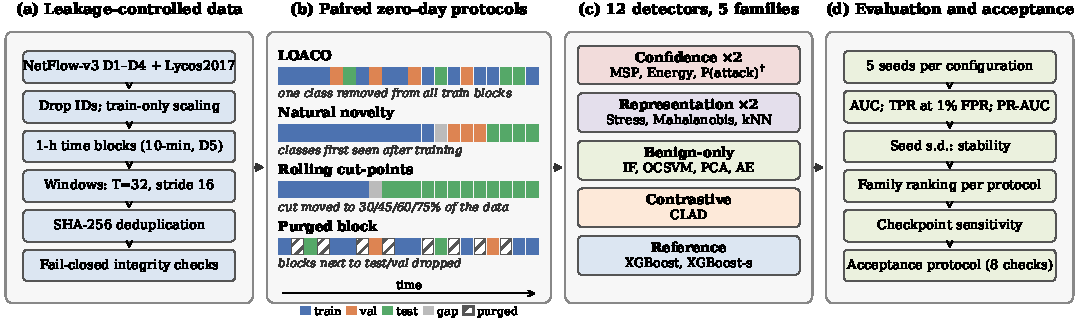
\includegraphics[width=\textwidth]{fig_overview.pdf}
\caption{HoNE overview. (a) Flows are grouped into time blocks before windowing and deduplicated, and every build runs fail-closed integrity checks. (b) Each detector is evaluated under class hold-out (LOACO) and natural temporal novelty, plus four rolling cut-points and a purged-block split for short captures. (c) Twelve detectors in five families, with confidence and representation scores recomputed on a GRU backbone and a seeded XGBoost-s, are scored on the same windows ($\dagger$: added after the final gate). (d) Results are reported per class over five seeds, with AUC, TPR at 1\% FPR, seed variability and family rankings, and condensed into the eight-check HoNE acceptance protocol.}
\label{fig:overview}
\end{figure*}

Applying HoNE to five public datasets yields six findings, each stated as an operator concern:
\begin{itemize}
\item \textbf{The standard test is often impossible on realistic captures.} Day-scheduled captures are known to place each attack on its own days~\cite{sharafaldin2018,moczkodan2026}; we quantify the consequence: temporal LOACO yields zero feasible folds on CIC-IDS2018, ToN-IoT and Lycos2017, while natural novelty offers 2--5 evaluable classes per split and 45 class--cut units over four rolling cut-points (Sec.~\ref{sec:c1}).
\item \textbf{The protocol picks the winner.} The leading detector family changes with dataset, protocol and cut-point, identically on both backbones. A gradient-boosted tree matches or beats the best novelty family in four of seven fixed evaluations, but trails benign-only detectors over the rolling cuts (Sec.~\ref{sec:c2}).
\item \textbf{One training run is not evidence.} Natural novelty raises the seed variability of the first backbone's scores by 1.7--17$\times$ relative to LOACO and of the GRU's representation scores by 2.6$\times$ (Sec.~\ref{sec:c3}).
\item \textbf{Some scores are invalid by construction.} Max-softmax and energy fall below chance in binary NIDS on both backbones, while the attack probability does not (Sec.~\ref{sec:c4}).
\item \textbf{AUC overstates zero-day coverage.} Over the rolling cuts no family catches more than 18\% of novel attack windows at 1\% false-positive rate, although family AUCs reach 0.75 (Sec.~\ref{sec:c6}).
\item \textbf{Shift effects are dataset-specific.} Temporal splits degrade one dataset severely and leave others intact, and zero-shot transfer is near chance (Sec.~\ref{sec:c5}).
\end{itemize}
Sec.~\ref{sec:related} reviews existing approaches and the gap they leave. Sec.~\ref{sec:method} derives HoNE's requirements and design, Sec.~\ref{sec:eval} reports the evaluation, Sec.~\ref{sec:disc} interprets the findings and presents the acceptance protocol, and Sec.~\ref{sec:concl} concludes.

\section{Related Work}
\label{sec:related}
Prior work on learned NIDS evaluation falls into four lines: studies of evaluation pitfalls, zero-day and open-set detectors, cross-domain studies, and sequence-based detectors. Each contributes a piece of what an operator needs, and each leaves a different piece missing.

\textbf{Evaluation pitfalls and datasets.} Arp et~al.\ catalogued ten pitfalls in security ML, including data snooping and inappropriate baselines~\cite{arp2022}; Apruzzese et~al.\ showed that ML-NIDS evaluations rarely reflect operational assumptions~\cite{apruzzese2023sok}; and dataset audits found flow-construction and labelling errors in CIC-IDS2017~\cite{engelen2021,rosay2021} and Pinto et~al.\ reviewed the tools and processes used to build NIDS datasets and their drawbacks~\cite{pinto2025}. The NetFlow standardization of Sarhan et~al.\ made datasets comparable~\cite{sarhan2021netflow,sarhan2022standard}, and its third version adds per-flow timestamps~\cite{luay2025}. These works diagnose \emph{how} evaluations go wrong, but they do not compare zero-day protocols or measure what the pitfalls do to detector rankings.

\textbf{Zero-day and open-set detection.} Zoppi et~al.\ found that unsupervised meta-learning ensembles detect simulated unknown attacks better than other algorithm families~\cite{zoppi2023}, and Sarhan et~al.\ linked low zero-day detection rates to distribution distance~\cite{sarhan2023zeroshot}. Recent detectors instead train with known attacks: CLAD learns benign structure with a contrastive loss~\cite{wilkie2026}, and Jodayree et~al.\ combine a transformer with energy scoring and extreme-value calibration~\cite{jodayree2026}. These studies measure zero-day ability, but all of them use class hold-out, usually without reporting seed variability, so their conclusions inherit LOACO's assumptions.

\textbf{Temporal and protocol-aware evaluation.} Time-aware evaluation changed conclusions in malware detection~\cite{pendlebury2019} and intrusion detection under drift~\cite{andresini2021}, and multi-period benchmarks such as AnoShift~\cite{dragoi2022} and MAWIFlow~\cite{schraven2026} test detectors on traffic from later years. For zero-day detection, ThreatFormer-IDS splits ToN-IoT in time and then removes chosen attack families from training, reporting five seeds and recall at 1\% FPR for a single model~\cite{nayak2026}; Alhalangy and Eltayeb combine chronological splits with leave-one-attack-family-out for one proposed detector~\cite{alhalangy2026}; Mesca et~al.\ compare random, attack-held-out and leave-one-out protocols on industrial traffic~\cite{mesca2026}; and Raj et~al.\ report future-time and leave-one-attack-type-out tests on RPL-IoT~\cite{raj2026}. Others show that chronological splits on day-scheduled CIC-IDS2017 degenerate~\cite{moczkodan2026}, that the way capture days are assembled reverses detector orderings~\cite{youssef2026}, that temporal splits on ToN-IoT change classifier rankings~\cite{abdessamad2026}, and that timestamp fields leak the attack schedule~\cite{sakr2026}. None of these pairs random-split LOACO with naturally novel classes on the same detectors and seeds, compares seed variability between protocols, or moves the training origin and scores only the classes that are new at each cut.

\textbf{Confidence scores for unknown attacks.} Confidence-based out-of-distribution scores are weaker on binary than on multi-class NIDS models~\cite{corsini2023}, softmax baselines scored below chance on held-out attacks in multi-class NIDS~\cite{zhang2021}, softmax entropy and energy trailed uncertainty-aware models~\cite{talpini2024}, and deep open-set recognition has been benchmarked for NIDS at NOMS~\cite{baye2023}. In contrast to Mesca et~al., who sign-flip ensemble members whose attack probability falls below chance~\cite{mesca2026}, we find the attack probability valid and MSP and energy inverted, and give a short derivation of why.

\textbf{Cross-domain generalization.} Layeghy and Portmann~\cite{layeghy2023xdomain}, DI-NIDS~\cite{layeghy2023dinids}, Cantone et~al.~\cite{cantone2024} and recent work on flow-based IoT detection~\cite{martinez2026} show that detectors degrade sharply on networks other than the one they were trained on. This line addresses shift \emph{between} networks, whereas an operator's first concern is shift \emph{over time within} the network being protected.

\textbf{Research gap and positioning.} Taken together, these lines leave one question unanswered: does the hold-out evidence used to support zero-day claims agree with how detectors behave under natural temporal novelty, on the same detectors, data and seeds? Answering it requires leakage control, paired protocols, a broad detector panel and variability reporting at once. HoNE provides all four, and it differs from prior benchmarks in treating the evaluation protocol itself as the object of study; to our knowledge it is also the first pre-registered NIDS benchmark.\ifappendix\ Appendix~\ref{app:related} extends this review to sequence, neuromorphic and drift-aware NIDS and positions HoNE against prior work in Table~\ref{tab:pos}.\fi

\section{Methodology}
\label{sec:method}
This section first derives the requirements that a trustworthy zero-day evaluation must meet, then describes how each HoNE component implements one of them.

\subsection{Requirements}
The gap in Sec.~\ref{sec:related} translates into four requirements. \textbf{R1, leakage control:} near-duplicate windows and attack episodes must not span training and test sets. \textbf{R2, protocol pairing:} every detector must be scored under both LOACO and natural temporal novelty on the same data and seeds, and infeasible protocols must be reported rather than silently skipped. \textbf{R3, score breadth and validity:} detectors from different families, including simple baselines, must be compared, and each score must be meaningful for a binary detector. \textbf{R4, variability and accountability:} results must be reported over several seeds with per-class variability, and protocol changes must be recorded. HoNE's four components map one-to-one onto these requirements (Fig.~\ref{fig:overview}a--d).

\subsection{Leakage-controlled data (R1)}
\textbf{Input data.} HoNE takes public flow-level datasets with per-flow timestamps as input. All five are downloaded from their official sources, registered with their SHA-256, size, row count and column list before use, and never modified (Table~\ref{tab:data}).

\emph{NetFlow-v3 datasets (D1--D4).} D1--D4 are the NetFlow-v3 versions of CSE-CIC-IDS2018~\cite{sharafaldin2018}, UNSW-NB15~\cite{moustafa2015}, ToN-IoT~\cite{moustafa2021} and BoT-IoT~\cite{koroniotis2019}. The dataset maintainers re-extracted each testbed's original packet captures into one common NetFlow schema of 53 features (byte and packet counts, durations, TCP flags, packet-size bins, throughput and inter-arrival statistics) with millisecond flow start and end timestamps~\cite{sarhan2021netflow,luay2025}. Every flow carries a binary label and an attack-class label. The captures span 14~Feb--2~Mar 2018 (D1, 14 attack labels), 22~Jan--18~Feb 2015 (D2, 9 classes), 23--29~Apr 2019 (D3, 9 classes) and May--Jun 2018 (D4, 4 classes).

\emph{Lycos2017 (D5).} D5 is a re-extraction of the CIC-IDS2017 packet captures (3--7~Jul 2017) with a corrected flow builder and corrected labels~\cite{rosay2021,engelen2021}. We run the authors' labelling script unmodified on their released flows and then apply a fixed adapter: microsecond timestamps become millisecond flow start times, the label becomes the attack class and a binary label, address and port columns are mapped to the identifier fields that HoNE drops, and the flow ID is removed. D5 keeps its own feature space (73 features after cleaning) and is therefore not used for cross-dataset transfer.

\emph{Labels and roles.} D1's 14 file labels are grouped into six attack families (bot, brute force, DDoS, DoS, infiltration, web attacks), following the families published by the dataset maintainers, so that a held-out class has no near-identical sibling in training (e.g., DoS-Hulk when DoS-GoldenEye is held out). The mapping is checked automatically: every label is assigned exactly once, and family totals reproduce the published counts. D4 contains only 1,315 benign windows and serves only as a transfer target.

\emph{Audit.} Before processing, every file is audited for row and column counts, conformity to the expected schema, missing and infinite values, consistency between the binary and class labels, and timestamp range. No file lacked a schema column or had a label conflict; D2 and D4 contain missing and infinite values, which are imputed as described below.

\begin{table}[!t]
\centering\scriptsize\setlength{\tabcolsep}{3pt}
\caption{Datasets. Windows are counted before deduplication.}
\label{tab:data}
\begin{tabular}{llrrrl}
\toprule
ID & Dataset & Flows & Windows & Dupl. & Classes\\
\midrule
D1 & NF-CIC-IDS2018-v3 & 20.1\,M & 1,257,018 & 1,838 & 14 (6 fam.)\\
D2 & NF-UNSW-NB15-v3 & 2.37\,M & 147,801 & 0 & 9\\
D3 & NF-ToN-IoT-v3 & 27.5\,M & 1,719,860 & 166,669 & 9\\
D4 & NF-BoT-IoT-v3 & 16.9\,M & 1,058,314$^{a}$ & 167,462 & 4\\
D5 & Lycos2017 & 1.84\,M & 114,783 & 0 & 13\\
\bottomrule
\multicolumn{6}{l}{$^{a}$D4 has no split of its own (transfer target only).}
\end{tabular}
\end{table}

\textbf{Processing.} To meet R1, every dataset then passes through the same steps (Fig.~\ref{fig:overview}a).
(1)~\emph{Drop identifiers:} addresses, ports and DNS query IDs are removed, because they identify hosts rather than behaviour, and TTL fields are removed as a known UNSW-NB15 label-leakage artifact; timestamps are kept only for ordering and splitting.
(2)~\emph{Order and block:} flows are sorted by start time (ties broken by original row order) and cut into contiguous 1-hour blocks (10-minute blocks for D5's purged split).
(3)~\emph{Window:} windows of $T{=}32$ consecutive flows with stride 16 are cut \emph{inside} blocks, so no window crosses a block. A window is an attack if any of its flows is, its class is the majority attack class, and a class-presence mask records every class it contains, so that a LOACO fold can exclude every window holding \emph{any} flow of the held-out class.
(4)~\emph{Deduplicate:} each window is hashed (SHA-256 of its raw feature values) and only the earliest copy of an exact duplicate is kept, across the whole dataset; this removed 9.7\% of D3's and 15.8\% of D4's windows.
(5)~\emph{Split:} whole blocks, never single flows or windows, are assigned to training, validation and test sets (Sec.~\ref{sec:protocols}).
(6)~\emph{Clean with training statistics only:} infinite values become missing and are imputed with the training median, non-negative heavy-tailed counts are $\log(1{+}x)$-transformed, zero-variance features and one of each pair with $|r|\geq0.999999$ are removed, and features are standardized with training means and deviations. Intersecting the features kept on D1--D3 leaves 41 common features; transfer targets, including D4, are transformed with the source dataset's cleaner, so nothing is fitted on target data.

Because a silent leakage bug would invalidate every later result, each build runs fail-closed integrity checks covering hash- and block-level disjointness of splits, class ratios, the absence of held-out flows from LOACO training sets, and finite values. All passed, including 538 checks on the D1--D4 archives after Amendment~1 and 32 on the D5 purged-block build.

\subsection{Paired zero-day protocols (R2)}
\label{sec:protocols}
On these leakage-controlled windows, HoNE defines two splits and four protocols. \emph{grouped\_random} shuffles blocks 60/20/20 into training, validation and test sets, and \emph{temporal\_gap} orders them in time, with the first 60\% for training, one discarded gap block, then 20\% each for validation and test. \emph{LOACO} runs on grouped\_random: a class is eligible if its training pool holds at least 200 windows (by majority label), and it is evaluated only if it also occurs in the test split. \emph{Natural novelty} runs on temporal\_gap and scores the classes that occur in test but never in training; its validation set is the last 20\% of the training period, because otherwise some datasets have attacks in every validation window. For short captures, the \emph{purged-block} split assigns 10-minute blocks 60/20/20 within each capture day and removes blocks adjacent to test or validation blocks, following purged cross-validation~\cite{lopezdeprado2018}; its folds additionally require 50 test windows. \emph{Rolling cut-points} (Amendment~7) re-apply the natural-novelty rule with the training period ending at 30, 45, 60 and 75\% of each dataset's windows, one discarded gap block, and testing on everything after; the cleaner is refitted on each cut's training rows, and each (dataset, cut, class) is one unit. Training sets are balanced 1:1 (7,000 windows per class), and validation and test sets use a 5:1 benign-to-attack ratio.

\subsection{Detector panel (R3)}
Meeting R3 requires detectors that read different evidence, so HoNE groups 12 scores into five families by what they read from a model, adapted from the taxonomy of~\cite{yang2024ood} (Table~\ref{tab:det}). \emph{Confidence} scores read the classifier output; \emph{representation-distance} scores read hidden features~\cite{lee2018,sun2022knn}; \emph{benign-only} detectors never see attacks~\cite{liu2008,scholkopf2001}; the \emph{contrastive} detector CLAD~\cite{wilkie2026} is trained on benign and known attacks; and XGBoost~\cite{chen2016} on flattened windows is a supervised reference. Higher scores always mean more anomalous, and orientation was fixed before any run.

\begin{table}[!t]
\centering\scriptsize\setlength{\tabcolsep}{2.5pt}
\caption{Twelve detectors in five families, plus a seeded XGBoost-s; confidence and representation scores are also computed on a GRU backbone.}
\label{tab:det}
\begin{tabular}{lll}
\toprule
Family & Detectors & Fitted on\\
\midrule
Confidence & MSP~\cite{hendrycks2017}, Energy~\cite{liu2020energy}, $P(\text{attack})^\dagger$ & Backbone output\\
Representation & Stress, Mahalanobis~\cite{lee2018}, $k$NN~\cite{sun2022knn} & Backbone features\\
Benign-only & IF~\cite{liu2008}, OCSVM~\cite{scholkopf2001}, PCA, autoencoder & Benign windows\\
Contrastive & CLAD~\cite{wilkie2026} & Benign + attacks\\
Reference & XGBoost~\cite{chen2016}, XGBoost-s & Labelled windows\\
\bottomrule
\end{tabular}
\end{table}

Confidence and representation scores come from a recurrent backbone (AHSD) built around a fixed benign reference $E$. Each flow vector is embedded as $z_t=\mathrm{LayerNorm}(Wx_t)\in\mathbb{R}^{128}$, and a state $h_t$, initialised at $E$, tracks the input relative to it with per-step, per-channel gates:
\begin{equation}
h_t = h_{t-1} + \alpha_t\odot(z_t - E) - \beta_t\odot(h_{t-1}-E),
\end{equation}
with gates $[\alpha_t,\beta_t]=\sigma(W_g[z_t,h_{t-1}])$.
$E$ is not learned: it is the mean embedding of benign training windows, tracked by an exponential moving average during training and set exactly afterwards. Stress $=\frac{1}{TD}\sum_{t,d}|h_{t,d}-E_d|$, and a two-layer head (linear--GELU--linear) reads $[h_T,\ \frac{1}{T}\sum_t h_t,\ \text{stress}]$ and outputs $P(\text{attack})$; its hidden layer is the representation used by Mahalanobis and $k$NN. To test whether findings depend on this backbone, every confidence and representation score is recomputed on a second backbone, a one-layer GRU (hidden size 128) with the same embedding and head (without stress), trained identically (Amendment~7). XGBoost uses subsample and column sampling of 1 and is therefore deterministic; XGBoost-s uses 0.8 for both with the run's seed, so that the stability comparison is not made against a deterministic baseline.

The validity part of R3 matters most for the confidence family. In a two-class detector with logit margin $\Delta=f_{\text{attack}}-f_{\text{benign}}$, MSP $=\max(P(\text{attack}),\,1-P(\text{attack}))=\sigma(|\Delta|)$ measures how \emph{sure} the model is, not \emph{which} class it chose; temperature calibration rescales $\Delta$ and cannot change this ranking. A new attack that the classifier detects confidently has MSP close to 1, so the anomaly score $1-\text{MSP}$ is close to 0 and the attack reads as in-distribution; energy behaves the same way because it decreases as the largest logit grows. This short derivation, not an empirical discovery, explains the inversion; HoNE therefore reports $P(\text{attack})$ alongside MSP and energy; because it was added after the final pre-registered gate (marked $\dagger$), comparisons involving it are diagnostic rather than confirmatory.

\subsection{Variability and accountability (R4)}
\label{sec:prereg}
Every configuration is run with five seeds, and results are reported per class with their seed standard deviation, so that run-to-run variation is visible rather than averaged away. Besides ROC AUC we report the true-positive rate at 1\% false-positive rate (TPR@1\%), the quantity a security team experiences, and PR-AUC. To keep protocol changes accountable, research questions, metrics and gates were written to a file and hashed before each experiment, and every result records that hash, the code commit and the dataset hashes~\cite{nosek2018}. Seven dated amendments are recorded. Amendments~1 and~5 changed protocols after data-only feasibility counts showed a rule could not be met; Amendments~2--4 each followed a STOP verdict and defined a new pilot and gate; Amendment~6 turned the study into a descriptive benchmark after the fourth STOP and recorded a flaw in the last gate's contrast; and Amendment~7, written after an independent read of the draft and before any run it governs, added the GRU backbone, XGBoost-s, rolling cut-points and operating-point metrics, with every result reported whatever it showed. Every amendment was hashed before the runs it governed, and none changed a recorded verdict.

\section{Evaluation}
\label{sec:eval}
We first describe the evaluation setup and then answer six questions, one per finding in Sec.~\ref{sec:intro}.

\subsection{Evaluation setup}
Both backbones are trained with AdamW (learning rate $10^{-3}$, weight decay $10^{-4}$), cosine annealing, gradient clipping at 1.0, batch size 256 and 15 epochs; the best validation macro-F1 checkpoint is kept (CLAD: best validation AUROC), and every evaluation is repeated with the final-epoch checkpoint. Seeds are 17, 23, 42, 101 and 202, and a seeding regression test runs before every experiment. We report ROC AUC, TPR@1\% and PR-AUC per detector and class (mean over seeds, Student-$t$ 95\% interval, seed standard deviation) and per family (mean over detectors and classes, with a paired bootstrap over classes and seeds, 2,000 resamples). The 1\% threshold is set on each test set's benign windows, so TPR@1\% is descriptive. Intervals are descriptive. All 210 final runs (Amendment~7) used one code commit and include the 160 runs of Amendment~6, whose results they reproduce exactly; reports are regenerated from stored result files only. Compute: a CPU-only cloud container (4 vCPUs, Intel Xeon at 2.10\,GHz, no GPU); the 210 runs took 10.8\,h (185\,s per run, both backbones and all detectors). Artifact: \artifact.

\subsection{Is LOACO feasible on realistic captures?}
\label{sec:c1}
The first question is whether the standard protocol can even be run once leakage is controlled. Temporal LOACO yields no feasible folds on any of the three day-scheduled captures (D1, D3, D5); only D2, which interleaves attacks in time, supports it (Table~\ref{tab:feas}). In D1 and D3 each attack class occupies its own days, so a time-ordered split places a class wholly in training or wholly in test. On D5 the purged split kept 125 of 219 blocks, and only one class (dos\_hulk) met both thresholds; web brute force had 199 training windows. Natural novelty, by contrast, offers two to five evaluable classes on every day-scheduled capture, and moving the cut-point multiplies this evidence to 45 units over 19 unique classes, 15 per dataset (D2 has no test-only class at any cut, and D3 no benign validation windows at a 30\% cut). This makes the comparison in the next question possible.

\begin{table}[!t]
\centering\footnotesize\setlength{\tabcolsep}{3pt}
\caption{Feasible zero-day evaluations per dataset (LOACO folds; natural-novelty classes; rolling class--cut units with feasible cuts out of 4).}
\label{tab:feas}
\begin{tabular}{lcccc}
\toprule
Dataset & Grouped & Temporal & Natural & Rolling\\
\midrule
D1 CIC-IDS2018 & 6 & 0 & 2 & 15 (4)\\
D2 UNSW-NB15 & 8 & 8 & 0 & 0 (0)\\
D3 ToN-IoT & 6 & 0 & 5 & 15 (3)\\
D5 Lycos2017 & 0$^{a}$ & 0 & 2 & 15 (3)\\
\midrule
\multicolumn{5}{l}{$^{a}$One fold under the purged-block split.}\\
\bottomrule
\end{tabular}
\end{table}

\subsection{Does the protocol change the winner?}
\label{sec:c2}
Given that both protocols can be run on some datasets, the next question is whether they agree. They do not (Table~\ref{tab:fam}). Representation-distance scores lead in five evaluations and benign-only detectors in two. The sharpest reversal is on D3: under LOACO, benign-only and representation scores are close ($+0.022$ [$+0.004$, $+0.047$]), whereas under natural novelty benign-only detectors lead by $+0.376$ [$+0.247$, $+0.500$] and representation scores fall to chance. CLAD never leads; it trails benign-only detectors on both D3 evaluations ($-0.123$ and $-0.075$) and is below 0.5 on every seed for D3 LOACO ddos. XGBoost exceeds the leading novelty family on LOACO D2 and natural novelty D3 and D5, and ties it on purged D5, while natural novelty D1 is hard for every family. The GRU backbone selects the same leading family as AHSD in all seven evaluations, so the reversal is not an artifact of one backbone; its absolute values can differ, however (natural novelty D3: GRU representation 0.869 against AHSD's 0.522, still below benign-only detectors at 0.898).

Pooling every class of each protocol shows the effect at a glance (Fig.~\ref{fig:winners}): representation scores win under LOACO, XGBoost under natural novelty, and benign-only detectors over the rolling cut-points. Over the 45 rolling units, benign-only detectors lead (0.748 [0.699, 0.796]) ahead of representation scores (0.623 [0.566, 0.683]; difference $+0.125$ [$+0.048$, $+0.204$]), and XGBoost trails the leading family by $-0.076$ [$-0.154$, $-0.009$]; at a 45\% cut on D3 it scores 0.263, below chance. The leader also moves with the dataset (representation on D1 and D5, benign-only on D3) and with the cut fraction (representation, benign-only, CLAD, benign-only from 30\% to 75\%). A detector chosen on one protocol, dataset or cut-point can therefore be the wrong choice on another.

\begin{figure}[!t]
\centering
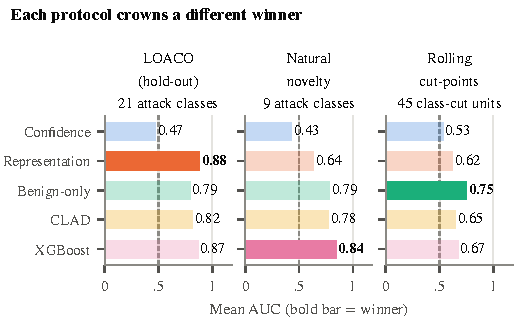
\includegraphics[width=\columnwidth]{fig_winners.pdf}
\caption{Mean AUC per detector family pooled over all classes of each protocol (rolling: all 45 class--cut units). The winner (solid bar) differs in each protocol; XGBoost is included as a supervised reference.}
\label{fig:winners}
\end{figure}

\begin{table}[!t]
\centering\footnotesize\setlength{\tabcolsep}{2.4pt}
\caption{Family mean AUC (five seeds). Bold: leading novelty family. Conf.\ = confidence, Repr.\ = representation, Benign = benign-only. Classes per evaluation in parentheses.}
\label{tab:fam}
\begin{tabular}{lccccc}
\toprule
Evaluation & Conf. & Repr. & Benign & CLAD & XGB\\
\midrule
LOACO D1 (6) & .553 & \textbf{.729} & .660 & .653 & .682\\
LOACO D2 (8) & .439 & \textbf{.977} & .807 & .949 & .998\\
LOACO D3 (6) & .426 & .881 & \textbf{.903} & .780 & .862\\
Purged D5 (1) & .580 & \textbf{.998} & .833 & .972 & 1.00\\
Natural D1 (2) & .529 & \textbf{.623} & .505 & .574 & .523\\
Natural D3 (5) & .467 & .522 & \textbf{.898} & .823 & .923\\
Natural D5 (2) & .256 & \textbf{.940} & .794 & .864 & .968\\
\bottomrule
\end{tabular}
\end{table}

\subsection{Is one training run enough evidence?}
\label{sec:c3}
A change of winner could still be a matter of noise, so the third question is how much results vary across seeds. On the first backbone, every stochastic supervised score (the six backbone scores and CLAD) is less stable under natural novelty than under LOACO (Table~\ref{tab:sd}). The effect is smaller on the GRU: its representation scores become 2.6$\times$ less stable, its confidence scores 1.0--1.3$\times$. Seeding XGBoost (XGBoost-s) raises its seed standard deviation only to 0.014, so the instability belongs to learned representations under shift rather than to seeding as such, and its size depends on the backbone. The seeded benign-only detectors (Isolation Forest, autoencoder) stay below 0.018 seed standard deviation under natural novelty, below every supervised score's minimum of 0.074; OCSVM, PCA and XGBoost are deterministic and carry no evidence about stability. On D3 natural novelty, $k$NN has a seed standard deviation of 0.33--0.40 AUC on four of five classes, so the same detector can rank first or last depending on the seed. Fig.~\ref{fig:d3} shows this on the three D3 classes evaluated under both protocols.

\begin{table}[!t]
\centering\footnotesize\setlength{\tabcolsep}{4pt}
\caption{Mean seed standard deviation of AUC. LOACO pools D1--D3; natural novelty pools D1, D3, D5. GRU rows: second backbone; XGBoost-s: seeded XGBoost.}
\label{tab:sd}
\begin{tabular}{llccc}
\toprule
Detector & Family & LOACO & Natural & Ratio\\
\midrule
MSP & Conf. & 0.061 & 0.103 & 1.7$\times$\\
Energy & Conf. & 0.055 & 0.100 & 1.8$\times$\\
$P(\text{attack})^\dagger$ & Conf. & 0.042 & 0.082 & 2.0$\times$\\
Stress & Repr. & 0.019 & 0.110 & 5.8$\times$\\
Mahalanobis & Repr. & 0.009 & 0.074 & 7.9$\times$\\
$k$NN & Repr. & 0.013 & 0.215 & 17.0$\times$\\
GRU Mahal. & Repr. & 0.008 & 0.022 & 2.6$\times$\\
GRU $k$NN & Repr. & 0.019 & 0.051 & 2.6$\times$\\
GRU MSP & Conf. & 0.049 & 0.062 & 1.3$\times$\\
GRU $P(\text{attack})$ & Conf. & 0.027 & 0.027 & 1.0$\times$\\
CLAD & Contr. & 0.020 & 0.058 & 2.9$\times$\\
XGBoost-s & Ref. & 0.006 & 0.014 & 2.4$\times$\\
Isolation Forest & Benign & 0.007 & 0.008 & 1.1$\times$\\
Autoencoder & Benign & 0.002 & 0.017 & 9.2$\times$\\
\bottomrule
\end{tabular}
\end{table}

\begin{figure}[!t]
\centering
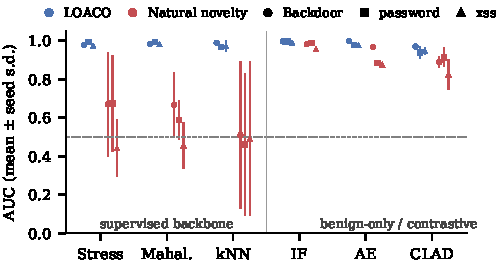
\includegraphics[width=\columnwidth]{fig_d3.pdf}
\caption{D3 (ToN-IoT) classes evaluated under both protocols: mean AUC $\pm$ seed standard deviation over five seeds. Supervised-backbone scores are tight under LOACO and spread widely under natural novelty; benign-only detectors stay tight. Dashed line: chance.}
\label{fig:d3}
\end{figure}

\subsection{Which novelty scores are valid?}
\label{sec:c4}
The confidence family scored worst in Table~\ref{tab:fam}, and Sec.~\ref{sec:method} predicted why. MSP and energy fall below 0.5 wherever the classifier detects unseen attacks confidently (Table~\ref{tab:conf}). On LOACO D2, MSP is below 0.5 on every seed of all eight classes while $P(\text{attack})$ reaches 0.997--1.000 on the same models: the classifier detects the held-out attacks, and MSP reads that confidence as normality. The GRU repeats the pattern (LOACO D2: MSP 0.162 vs $P(\text{attack})$ 0.999; natural novelty D3: 0.245 vs 0.918), and in-distribution MSP is 0.065--0.340 on grouped D1--D3 splits. Across all 34 evaluation--backbone pairs, MSP exceeds $P(\text{attack})$ only in five rolling cuts where $P(\text{attack})$ is itself at or near chance (0.345--0.548), i.e.\ where the classifier misses the novel class. $P(\text{attack})$ falls below 0.5 only on individual classes (D3 LOACO ddos 0.35 and scanning 0.46; D5 portscan 0.16). Representation distance is valid on average, but on natural novelty D3 its interval [0.402, 0.647] includes 0.5. As noted in Sec.~\ref{sec:method}, the $P(\text{attack})$ comparisons are diagnostic; the inversion itself follows from the binary formulation.

\begin{table}[!t]
\centering\footnotesize\setlength{\tabcolsep}{4pt}
\caption{Mean AUC of confidence scores and the representation family.}
\label{tab:conf}
\begin{tabular}{lcccc}
\toprule
Evaluation & MSP & Energy & $P(\text{attack})^\dagger$ & Repr.\\
\midrule
LOACO D2 & 0.163 & 0.155 & 0.999 & 0.977\\
LOACO D3 & 0.269 & 0.258 & 0.752 & 0.881\\
Natural D3 & 0.262 & 0.287 & 0.853 & 0.522\\
Natural D5 & 0.103 & 0.090 & 0.575 & 0.940\\
\bottomrule
\end{tabular}
\end{table}

\subsection{How do temporal and cross-network shifts behave?}
\label{sec:c5}
Natural novelty mixes a new attack class with temporal shift, so the last question isolates the shift itself. Its effects are dataset-specific (Table~\ref{tab:temp}). On D1 both models lose 0.27--0.29 AUC under the temporal split; on D2 neither changes by more than 0.014; and on D5 both improve. Only on D3 does the AHSD backbone degrade (0.664, seed s.d.\ 0.202) while XGBoost holds 0.978; the GRU degrades less (0.981$\rightarrow$0.857), so the size of this drop depends on the backbone. Across 108 zero-shot transfer cells (12 detectors $\times$ 9 source--target pairs among D1--D4), the median AUC is 0.500 and 67\% fall in [0.3, 0.6]\ifappendix\ (Table~\ref{tab:a_transfer})\fi. Checkpoint choice moves representation and CLAD family means by at most 0.073 and confidence scores by up to 0.205 (D5, 26 validation attack windows).

\begin{table}[!t]
\centering\footnotesize\setlength{\tabcolsep}{4pt}
\caption{In-distribution AUC, grouped vs.\ temporal split.}
\label{tab:temp}
\begin{tabular}{lcccc}
\toprule
 & \multicolumn{2}{c}{$P(\text{attack})^\dagger$} & \multicolumn{2}{c}{XGBoost}\\
\cmidrule(lr){2-3}\cmidrule(lr){4-5}
Dataset & Grouped & Temporal & Grouped & Temporal\\
\midrule
D1 & 0.812 & 0.521 & 0.815 & 0.547\\
D2 & 0.999 & 0.997 & 0.998 & 0.984\\
D3 & 0.975 & 0.664 & 0.977 & 0.978\\
D5 & 0.831 & 0.948 & 0.705 & 0.990\\
\bottomrule
\end{tabular}
\end{table}

\subsection{Does AUC reflect detection at an operating point?}
\label{sec:c6}
An operator does not experience AUC but the share of attacks caught at a false-alarm rate the security team can absorb; base rates make this gap well known in principle~\cite{arp2022,apruzzese2023sok}, and some zero-day studies report recall at a fixed FPR~\cite{nayak2026,mesca2026}. Here we quantify it across protocols. The two disagree sharply (Fig.~\ref{fig:operating}). Under LOACO D2 the best families catch 87--99\% of held-out windows at 1\% false-positive rate. Under natural novelty D3, benign-only detectors reach an AUC of 0.90 but catch 12\%, and XGBoost 38\%. Over the 45 rolling units no family exceeds 18\% (XGBoost 0.18; benign-only 0.09 at AUC 0.75), and of the 333 detector--class points with AUC $\geq0.75$ under natural novelty, 184 catch fewer than 20\% of attack windows (median 0.15): novel attacks overlap the benign score tail.

\begin{figure}[!t]
\centering
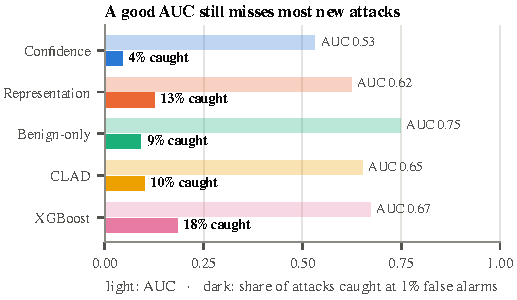
\includegraphics[width=\columnwidth]{fig_operating.pdf}
\caption{Rolling cut-points (45 units): each family's AUC (light bar) against the share of novel attack windows it catches at 1\% false-positive rate (dark bar).}
\label{fig:operating}
\end{figure}

\subsection{How do these results compare with published ones?}
\label{sec:prior}
Table~\ref{tab:prior} sets HoNE's numbers beside published results on the same datasets or questions. Metrics and dataset versions differ, so the table shows direction rather than a ranking. Class hold-out results in the literature (0.97--0.997 AUROC; 87--92\% zero-day detection) are matched by HoNE's LOACO numbers on D2 and D5, but the same detectors drop under natural novelty and rolling cuts: CLAD from 0.972 (purged D5) to 0.702 (rolling D5), and XGBoost on ToN-IoT from 0.862 (LOACO) to 0.699 (rolling). Softmax entropy and energy were reported at 0.76--0.80 AUROC for a multi-class detector on NF-ToN-IoT-v2~\cite{talpini2024}; on HoNE's binary detectors MSP and energy invert (0.26--0.27), as Sec.~\ref{sec:c4} predicts. ThreatFormer-IDS reports 78\% recall at 1\% FPR on held-out ToN-IoT families~\cite{nayak2026}, whereas no family reaches 20\% on HoNE's rolling units.

\begin{table*}[!t]
\centering\footnotesize\setlength{\tabcolsep}{3pt}
\caption{Previously reported results vs.\ HoNE on the same datasets or questions. Metrics, splits and dataset versions differ, so the comparison shows direction, not a like-for-like ranking.}
\label{tab:prior}
\begin{tabular}{llll}
\toprule
Setting & Source & Reported & HoNE\\
\midrule
Zero-day hold-out, UNSW-NB15 & \cite{sarhan2023zeroshot} & Z-DR 87--92\% (NF-v2) & LOACO D2: XGBoost 0.998, repr.\ 0.977 AUC\\
CLAD, LYCOS-IDS2017 & \cite{wilkie2026} & AUROC 0.997 & purged 0.972; natural 0.864; rolling 0.702\\
Held-out families, ToN-IoT & \cite{nayak2026} & AUROC 0.971; recall@1\%FPR 0.783 & best family: LOACO 0.903; rolling TPR@1\% $\leq$ 0.18\\
Softmax entropy / energy, NF-ToN-IoT & \cite{talpini2024} & AUROC 0.76 / 0.80 (multi-class) & LOACO D3: MSP 0.269, energy 0.258 (binary)\\
Random $\rightarrow$ temporal, TON-IoT & \cite{abdessamad2026} & macro-F1 0.87 $\rightarrow$ 0.58 & AUC: XGBoost 0.977 $\rightarrow$ 0.978, AHSD 0.975 $\rightarrow$ 0.664\\
Chronological split, CIC-IDS & \cite{moczkodan2026} & macro-F1 $\approx$ 0.50 & temporal D1 AUC: XGBoost 0.547\\
Cross-dataset transfer & \cite{cantone2024} & AUROC 0.59--0.82 & median 0.500 over 108 results\\
Unknown-attack recall & \cite{zoppi2023} & XGBoost Rec-Unk 0.38 & rolling XGBoost TPR@1\% 0.18\\
\bottomrule
\end{tabular}
\end{table*}

\subsection{Pre-registered negative results}
Before the benchmark became descriptive, four confirmatory hypotheses were tested against frozen gates, and all four failed\ifappendix\ (Appendix~\ref{app:neg})\fi: a spectral model of per-class detectability (pooled $\rho{=}0.326$, below 0.6); attack absorption by an adaptive equilibrium under supervised training (not reproduced; detectability peaks at a small adaptation rate); benign-drift re-anchoring (0 of 9 detectors met the improvement criterion); and benign-only superiority confined to natural novelty. The last gate's supervised family included MSP and energy, which Sec.~\ref{sec:c4} shows are invalid; the verdict stands as recorded.

\section{Discussion}
\label{sec:disc}
\textbf{Main findings.} The six questions give a consistent answer to the paper's operational question. On realistic captures, the standard zero-day test is often impossible; where it can be run, it can crown a different winner than natural novelty, and the winner moves again with the cut-point; single-run results can understate run-to-run variation by up to 17$\times$; and an AUC that looks adequate can mean that most novel attacks go unnoticed at an affordable false-alarm rate. A zero-day claim backed only by single-run LOACO on a random split therefore says little about how a detector will behave once deployed.

\textbf{Interpretation.} The protocols disagree because they change different things. LOACO keeps the benign traffic of the test period in training, so supervised representations place a held-out class far from benign traffic and distance scores excel (0.977 on D2). Under natural novelty the benign traffic itself shifts, and representations shaped by known attacks lose their reference point, which explains both the drop to chance and the seed dependence on D3; how far they fall depends on the backbone (GRU: 0.869). Benign-only detectors never depend on which attacks were trained on, which explains their stability, but not their accuracy: they lead on D3 natural novelty yet trail by 0.17 AUC on D2 LOACO. The strength of XGBoost on fixed evaluations is consistent with evidence that tree ensembles remain hard to beat on tabular data~\cite{grinsztajn2022}, and flattened flow windows are tabular data; its collapse at some cut-points shows that a supervised boundary can also place a new class on the wrong side.

\label{sec:protocol}
\textbf{What works: the HoNE acceptance protocol.} These mechanisms suggest what evidence does predict deployment behaviour, and the HoNE acceptance protocol asks an operator to require it before trusting a learned NIDS to detect zero-day attacks:
\begin{enumerate}
\item \textbf{Leakage controls stated:} time-block grouping before windowing, window deduplication, and purging for short captures.
\item \textbf{Natural novelty reported} wherever timestamps allow, next to LOACO, with an explicit statement when either is infeasible.
\item \textbf{Five or more seeds} with per-class seed standard deviation, not only means.
\item \textbf{No MSP or energy} as novelty scores for a binary detector; use $P(\text{attack})$ or a representation distance validated under natural novelty.
\item \textbf{Two baselines}: a benign-only detector and a gradient-boosted tree. In our benchmark XGBoost alone matched or exceeded the best novelty family in four of seven fixed evaluations, XGBoost or the benign-only family matched or exceeded every other family in five of seven, and benign-only detectors led over the rolling cut-points.
\item \textbf{Operating-point metrics}: TPR at the false-positive rate the security team can absorb, not only AUC.
\item \textbf{Checkpoint sensitivity} when validation sets are small.
\item \textbf{Pre-registration or a full amendment log}, including failed hypotheses.
\end{enumerate}
These checks cost little: each of our 210 final runs, covering two backbones and all detectors, took about three minutes on four CPU cores.

\textbf{Remaining limitations.} The protocol's evidence has limits that bound how far it generalizes. Both backbones are recurrent, so attention-based models may behave differently, and the size of the seed and temporal effects already differs between them. D1 and D5 contribute two natural-novelty classes each in the primary split; the rolling cuts add 45 units, but units of one class at several cuts share test windows and are not independent. D5's validation set holds only 26 attack windows. The 1-hour grouping, any-attack labelling, 200-window threshold and 5:1 test ratio were fixed in advance but are not the only reasonable choices; $P(\text{attack})$ was added post hoc; and CLAD was reimplemented from its paper, although it reaches 0.972 on purged D5, close to the 0.997 its authors report on the same dataset~\cite{wilkie2026} under their random-split protocol, so the comparison is only a sanity check of our reimplementation. Natural novelty is novel \emph{behaviour}; many real zero-days exploit new vulnerabilities with familiar behaviour~\cite{jibunoh2026}, which no flow benchmark captures. Finally, all datasets come from testbeds, and natural novelty follows the capture schedule, which is closer to deployment than LOACO but is not live traffic.

\textbf{Broader implications.} Within these limits, the findings matter beyond this benchmark. For network management, the acceptance protocol can be written into procurement: a vendor can be asked to report results on HoNE's released splits, under both protocols and over several seeds. For research, the results argue that zero-day claims should be accompanied by protocol-paired, multi-seed evidence, and that negative pre-registered results deserve publication, because they show where intuitive hypotheses about detector behaviour fail.

\section{Conclusion}
\label{sec:concl}
Operators must decide whether to trust learned NIDS on attacks that did not exist at training time, yet the evidence offered for such claims is usually a single LOACO run on a randomly split benchmark. We introduced HoNE, a pre-registered, leakage-controlled benchmark that scores every detector under both LOACO and natural temporal novelty, and applied it to five datasets, 12 detectors on two backbones and five seeds. Temporal LOACO proved infeasible on every day-scheduled capture; protocols, datasets and cut-points crowned different winners, on both backbones; natural novelty raised seed variability by up to 17$\times$; max-softmax and energy proved invalid for binary detectors; and AUCs up to 0.75 meant at most 18\% of novel attacks caught at 1\% false-positive rate. How zero-day detection is evaluated decides which detector looks best, so operators should ask for natural-novelty results at several cut-points, multiple seeds, valid scores, operating-point metrics and simple baselines before trusting a zero-day claim. We release HoNE's splits, amendments and code so that any detector can be evaluated under both protocols.

\bibliographystyle{IEEEtran}
\begin{thebibliography}{40}

\bibitem{wilkie2026}
J.~Wilkie, H.~Hindy, C.~Michie, C.~Tachtatzis, J.~Irvine, and R.~Atkinson, ``A novel contrastive loss for zero-day network intrusion detection,'' \emph{IEEE Trans. Netw. Service Manag.}, vol.~23, pp. 2064--2076, 2026.

\bibitem{jodayree2026}
M.~Jodayree, A.~Kavoosi~Ghafi, S.~Amiri, \emph{et al.}, ``Explainable zero-day attack detection in IoMT using transformer-based time-series modeling,'' \emph{Sci. Rep.}, vol.~16, Art. no. 23252, 2026.

\bibitem{arp2022}
D.~Arp, E.~Quiring, F.~Pendlebury, A.~Warnecke, F.~Pierazzi, C.~Wressnegger, L.~Cavallaro, and K.~Rieck, ``Dos and don'ts of machine learning in computer security,'' in \emph{Proc. 31st USENIX Security Symp.}, 2022, pp. 3971--3988.

\bibitem{engelen2021}
G.~Engelen, V.~Rimmer, and W.~Joosen, ``Troubleshooting an intrusion detection dataset: The CICIDS2017 case study,'' in \emph{Proc. IEEE Security and Privacy Workshops (SPW)}, 2021, pp. 7--12.

\bibitem{hendrycks2017}
D.~Hendrycks and K.~Gimpel, ``A baseline for detecting misclassified and out-of-distribution examples in neural networks,'' in \emph{Proc. Int. Conf. Learn. Represent. (ICLR)}, 2017.

\bibitem{liu2020energy}
W.~Liu, X.~Wang, J.~Owens, and Y.~Li, ``Energy-based out-of-distribution detection,'' in \emph{Proc. Adv. Neural Inf. Process. Syst. (NeurIPS)}, 2020, pp. 21\,464--21\,475.

\bibitem{sommer2010}
R.~Sommer and V.~Paxson, ``Outside the closed world: On using machine learning for network intrusion detection,'' in \emph{Proc. IEEE Symp. Security and Privacy (S\&P)}, 2010, pp. 305--316.

\bibitem{apruzzese2023sok}
G.~Apruzzese, P.~Laskov, and J.~Schneider, ``SoK: Pragmatic assessment of machine learning for network intrusion detection,'' in \emph{Proc. IEEE European Symp. Security and Privacy (EuroS\&P)}, 2023, pp. 592--614.

\bibitem{rosay2021}
A.~Rosay, F.~Carlier, E.~Cheval, and P.~Leroux, ``From CIC-IDS2017 to LYCOS-IDS2017: A corrected dataset for better performance,'' in \emph{Proc. IEEE/WIC/ACM Int. Conf. Web Intell. Intell. Agent Technol. (WI-IAT)}, 2021, pp. 570--575.

\bibitem{pinto2025}
D.~Pinto, I.~Amorim, E.~Maia, and I.~Pra\c{c}a, ``A review on intrusion detection datasets: Tools, processes, and features,'' \emph{Comput. Netw.}, vol.~262, Art. no. 111177, 2025.

\bibitem{sarhan2021netflow}
M.~Sarhan, S.~Layeghy, N.~Moustafa, and M.~Portmann, ``NetFlow datasets for machine learning-based network intrusion detection systems,'' in \emph{Big Data Technologies and Applications (BDTA 2020)}, LNICST, vol.~371. Springer, 2021, pp. 117--135.

\bibitem{sarhan2022standard}
M.~Sarhan, S.~Layeghy, and M.~Portmann, ``Towards a standard feature set for network intrusion detection system datasets,'' \emph{Mobile Netw. Appl.}, vol.~27, no.~1, pp. 357--370, 2022.

\bibitem{luay2025}
M.~Luay, S.~Layeghy, S.~Hosseininoorbin, M.~Sarhan, N.~Moustafa, and M.~Portmann, ``Temporal analysis of NetFlow datasets for network intrusion detection systems,'' arXiv:2503.04404, 2025.

\bibitem{zoppi2023}
T.~Zoppi, A.~Ceccarelli, T.~Puccetti, and A.~Bondavalli, ``Which algorithm can detect unknown attacks? Comparison of supervised, unsupervised and meta-learning algorithms for intrusion detection,'' \emph{Comput. Secur.}, vol.~127, Art. no. 103107, 2023.

\bibitem{sarhan2023zeroshot}
M.~Sarhan, S.~Layeghy, M.~Gallagher, and M.~Portmann, ``From zero-shot machine learning to zero-day attack detection,'' \emph{Int. J. Inf. Secur.}, vol.~22, no.~4, pp. 947--959, 2023.

\bibitem{layeghy2023xdomain}
S.~Layeghy and M.~Portmann, ``Explainable cross-domain evaluation of ML-based network intrusion detection systems,'' \emph{Comput. Electr. Eng.}, vol.~108, Art. no. 108692, 2023.

\bibitem{layeghy2023dinids}
S.~Layeghy, M.~Baktashmotlagh, and M.~Portmann, ``DI-NIDS: Domain invariant network intrusion detection system,'' \emph{Knowl.-Based Syst.}, vol.~273, Art. no. 110626, 2023.

\bibitem{martinez2026}
B.~A. Mart\'{\i}nez Gonz\'{a}lez, A.~D. Bermejo, M.~P\'{e}rez Sevilla, J.~A. Rinc\'{o}n Arango, and D.~Urda, ``Cross-domain generalization strategies for IoT cyberattack detection using flow-based features,'' \emph{Internet Things}, vol.~39, Art. no. 102044, 2026.

\bibitem{sharafaldin2018}
I.~Sharafaldin, A.~H. Lashkari, and A.~A. Ghorbani, ``Toward generating a new intrusion detection dataset and intrusion traffic characterization,'' in \emph{Proc. 4th Int. Conf. Inf. Syst. Secur. Privacy (ICISSP)}, 2018, pp. 108--116.

\bibitem{moustafa2015}
N.~Moustafa and J.~Slay, ``UNSW-NB15: A comprehensive data set for network intrusion detection systems,'' in \emph{Proc. Military Commun. Inf. Syst. Conf. (MilCIS)}, 2015, pp. 1--6.

\bibitem{moustafa2021}
N.~Moustafa, ``A new distributed architecture for evaluating AI-based security systems at the edge: Network TON\_IoT datasets,'' \emph{Sustain. Cities Soc.}, vol.~72, Art. no. 102994, 2021.

\bibitem{koroniotis2019}
N.~Koroniotis, N.~Moustafa, E.~Sitnikova, and B.~Turnbull, ``Towards the development of realistic botnet dataset in the Internet of Things for network forensic analytics: Bot-IoT dataset,'' \emph{Future Gener. Comput. Syst.}, vol.~100, pp. 779--796, 2019.

\bibitem{lopezdeprado2018}
M.~L\'{o}pez de Prado, \emph{Advances in Financial Machine Learning}. Hoboken, NJ, USA: Wiley, 2018.

\bibitem{yang2024ood}
J.~Yang, K.~Zhou, Y.~Li, and Z.~Liu, ``Generalized out-of-distribution detection: A survey,'' \emph{Int. J. Comput. Vis.}, vol.~132, no.~12, pp. 5635--5662, 2024.

\bibitem{lee2018}
K.~Lee, K.~Lee, H.~Lee, and J.~Shin, ``A simple unified framework for detecting out-of-distribution samples and adversarial attacks,'' in \emph{Proc. Adv. Neural Inf. Process. Syst. (NeurIPS)}, 2018, pp. 7167--7177.

\bibitem{sun2022knn}
Y.~Sun, Y.~Ming, X.~Zhu, and Y.~Li, ``Out-of-distribution detection with deep nearest neighbors,'' in \emph{Proc. 39th Int. Conf. Mach. Learn. (ICML)}, 2022, pp. 20\,827--20\,840.

\bibitem{liu2008}
F.~T. Liu, K.~M. Ting, and Z.-H. Zhou, ``Isolation forest,'' in \emph{Proc. 8th IEEE Int. Conf. Data Mining (ICDM)}, 2008, pp. 413--422.

\bibitem{scholkopf2001}
B.~Sch\"{o}lkopf, J.~C. Platt, J.~Shawe-Taylor, A.~J. Smola, and R.~C. Williamson, ``Estimating the support of a high-dimensional distribution,'' \emph{Neural Comput.}, vol.~13, no.~7, pp. 1443--1471, 2001.

\bibitem{chen2016}
T.~Chen and C.~Guestrin, ``XGBoost: A scalable tree boosting system,'' in \emph{Proc. 22nd ACM SIGKDD Int. Conf. Knowl. Discov. Data Min. (KDD)}, 2016, pp. 785--794.

\bibitem{nosek2018}
B.~A. Nosek, C.~R. Ebersole, A.~C. DeHaven, and D.~T. Mellor, ``The preregistration revolution,'' \emph{Proc. Natl. Acad. Sci. USA}, vol.~115, no.~11, pp. 2600--2606, 2018.

\bibitem{grinsztajn2022}
L.~Grinsztajn, E.~Oyallon, and G.~Varoquaux, ``Why do tree-based models still outperform deep learning on typical tabular data?'' in \emph{Proc. Adv. Neural Inf. Process. Syst. (NeurIPS), Datasets and Benchmarks Track}, 2022.

\bibitem{mirsky2018}
Y.~Mirsky, T.~Doitshman, Y.~Elovici, and A.~Shabtai, ``Kitsune: An ensemble of autoencoders for online network intrusion detection,'' in \emph{Proc. Netw. Distrib. Syst. Secur. Symp. (NDSS)}, 2018.

\bibitem{fernandez2026}
E.~Fern\'{a}ndez-Morales, J.~C. Garc\'{\i}a-Merino, L.~Tobarra, A.~Robles-G\'{o}mez, and R.~Pastor-Vargas, ``Deep learning approaches for intrusion detection in IoT environments: A systematic literature review,'' \emph{IEEE Internet Things J.}, 2026, doi: 10.1109/JIOT.2026.3719346.

\bibitem{manocchio2024}
L.~D. Manocchio \emph{et al.}, ``FlowTransformer: A transformer framework for flow-based network intrusion detection systems,'' \emph{Expert Syst. Appl.}, vol.~241, Art. no. 122564, 2024.

\bibitem{wang2024snn}
Z.~Wang, F.~A. Ghaleb, A.~Zainal, M.~M. Siraj, and X.~Lu, ``An efficient intrusion detection model based on convolutional spiking neural network,'' \emph{Sci. Rep.}, vol.~14, Art. no. 7054, 2024.

\bibitem{knapp2025}
L.~Knapp, S.~Nitzsche, M.~B\"{o}rsig, A.~Vasilache, I.~Baumgart, and J.~Becker, ``Efficacy of spiking neural networks for intrusion detection systems,'' in \emph{Proc. Int. Conf. Cybersecurity and AI-Based Systems (Cyber-AI)}, 2025, doi: 10.1109/Cyber-AI66431.2025.11233776.

\bibitem{liu2026netmasq}
Z.~Liu, Y.~Zhao, Z.~Liu, Q.~Li, C.~Fu, G.~Zhou, and K.~Xu, ``A hard-label black-box evasion attack against ML-based malicious traffic detection systems,'' in \emph{Proc. Netw. Distrib. Syst. Secur. Symp. (NDSS)}, 2026.

\bibitem{xu2026entente}
J.~Xu, C.~Li, Y.~Zheng, and Z.~Li, ``Entente: Cross-silo intrusion detection on network log graphs with federated learning,'' in \emph{Proc. Netw. Distrib. Syst. Secur. Symp. (NDSS)}, 2026.

\bibitem{depaola2026}
A.~De~Paola, S.~Drago, P.~Ferraro, and G.~Lo~Re, ``HOIDS: Concept drift aware hybrid online intrusion detection system,'' \emph{J. Netw. Comput. Appl.}, vol.~254, Art. no. 104556, 2026.

\bibitem{yang2021cade}
L.~Yang, W.~Guo, Q.~Hao, A.~Ciptadi, A.~Ahmadzadeh, X.~Xing, and G.~Wang, ``CADE: Detecting and explaining concept drift samples for security applications,'' in \emph{Proc. 30th USENIX Security Symp.}, 2021, pp. 2327--2344.

\end{thebibliography}

\ifappendix
\clearpage
\appendices

\section{Extended Related Work}
\label{app:related}
\textbf{Evaluation pitfalls.} Arp et~al.\ identified ten pitfalls in security ML, including data snooping and spurious correlations~\cite{arp2022}. Apruzzese et~al.\ argued that ML-NIDS research rarely supports operational assessment~\cite{apruzzese2023sok}. Sommer and Paxson explained why anomaly detection is harder outside a closed world~\cite{sommer2010}.

\textbf{Zero-day and open-set detection.} Kitsune detects anomalies with an ensemble of autoencoders trained on benign traffic~\cite{mirsky2018}. Wilkie et~al.\ (2026) learn benign structure from benign and known-malicious samples with a contrastive loss~\cite{wilkie2026}. Jodayree et~al.\ (2026) combine a protocol-aware transformer with energy scoring and extreme-value calibration~\cite{jodayree2026}. Both use class hold-out.

\textbf{Cross-domain generalization.} Beyond~\cite{layeghy2023xdomain,layeghy2023dinids,martinez2026}, a 2026 systematic review surveys deep IoT intrusion detection and its evaluation practice~\cite{fernandez2026}.

\textbf{Sequence and neuromorphic NIDS.} FlowTransformer provides a framework for transformer-based flow NIDS~\cite{manocchio2024}. Wang et~al.\ built a convolutional spiking detector~\cite{wang2024snn}, and Knapp et~al.\ evaluated bare spiking networks against conventional and recurrent networks~\cite{knapp2025}; both report in-distribution accuracy.

\textbf{Drift and adversaries.} At NDSS 2026, a reinforcement-learning attacker evaded six ML traffic detectors with only hard-label query access~\cite{liu2026netmasq}, and Entente addressed cross-silo detection on log graphs with federated learning~\cite{xu2026entente}. HOIDS combines online learning with drift awareness~\cite{depaola2026}, and CADE detects and explains drifting samples~\cite{yang2021cade}.

\begin{table}[!t]
\centering\scriptsize\setlength{\tabcolsep}{2pt}
\caption{Positioning. -- = not assessed in this comparison.}
\label{tab:pos}
\begin{tabular}{lllll}
\toprule
Work & Zero-day protocol & Cross-dataset & Seed var. & Pre-reg.\\
\midrule
\cite{sarhan2023zeroshot} & Zero-shot hold-out & No & -- & No\\
\cite{zoppi2023} & Simulated unknowns & No & -- & No\\
\cite{layeghy2023xdomain} & No & Yes & -- & No\\
\cite{wilkie2026} & LOACO & No & -- & No\\
\cite{nayak2026} & Time split + held-out families & No & 5 seeds (agg.) & No\\
\cite{alhalangy2026} & Chronological + LOAFO & No & 5 seeds (agg.) & No\\
\cite{mesca2026} & Random / held-out / LOO & No & -- & No\\
\cite{jodayree2026} & Leave-one-type-out & 1 pair & 5 seeds & No\\
HoNE & LOACO, natural, rolling, purged & 9 pairs & 5 seeds $\times$ 2 backb. & Yes\\
\bottomrule
\end{tabular}
\end{table}

\section{Pre-Registered Gates and Amendments}
\label{app:neg}
\begin{table}[!t]
\centering\scriptsize\setlength{\tabcolsep}{2pt}
\caption{Pre-registered gates. All four returned STOP.}
\label{tab:gates}
\begin{tabular}{p{0.06\columnwidth}p{0.30\columnwidth}p{0.27\columnwidth}p{0.27\columnwidth}}
\toprule
Gate & Hypothesis & Frozen criterion & Observed\\
\midrule
P1 & Spectral filter model predicts per-class detectability & Pooled $\rho\ge0.6$ and better than Wasserstein & $\rho{=}0.326$; difference CI [$-0.578$, 1.286]\\
G1 & Adaptive equilibrium absorbs attacks under supervised training & $\rho(\gamma,d')\le-0.8$ on $\ge$2 of 3 datasets & $-0.143$, $-0.143$, 0.000\\
G2 & Benign drift causes inversion; re-anchoring fixes it & $\ge$5 of 9 detectors pass each criterion & 4/9, 5/9, 0/9\\
G3 & Benign-only beats supervised only under natural novelty & $B{-}S\ge0.15$ natural; $\le0.05$ LOACO & $+0.191$ (D5); $+0.269$ (D3 LOACO)\\
\bottomrule
\end{tabular}
\end{table}

\textbf{Amendment log.} A1: LOACO moved to grouped\_random; D1 classes defined as families; D4 made a transfer target. A2: spectral predictor demoted to secondary; D1 natural novelty dropped (validation empty); new gate G1. A3: G1 negative; train-tail validation introduced, which restored D1 natural novelty; new gate G2. A4: G2 negative; Lycos2017 and CLAD added; new gate G3. A5: purged-block protocol for D5 with a pre-declared fallback; checkpoint sensitivity. A6: descriptive benchmark; gate flaw recorded; $P(\text{attack})$ added. A7 (after an independent read of the draft, before any run it governs): GRU backbone, seeded XGBoost-s, rolling cut-points and operating-point metrics; full rerun of 210 runs at one code commit.

\section{Per-Class and Transfer Results}
% generated by paper/hone/gen_appendix.py from results/final_v2/summary.json; do not edit
\begin{table}[!t]
\centering
\scriptsize
\setlength{\tabcolsep}{2.6pt}
\caption{Per-class AUC, LOACO D1 (CIC-IDS2018 families). Mean of five seeds; s.d.\ = mean seed standard deviation over classes.}
\label{tab:a_l1}
\begin{tabular}{lccccccc}
\toprule
Detector & Bot & Brute F. & DDoS & DoS & Infil. & Web & s.d.\\
\midrule
MSP & 0.67 & 0.50 & 0.51 & 0.28 & 0.49 & 0.66 & 0.093\\
Energy & 0.58 & 0.48 & 0.50 & 0.19 & 0.49 & 0.64 & 0.072\\
P(att.)$^\dagger$ & 0.73 & 0.71 & 0.51 & 0.84 & 0.52 & 0.66 & 0.103\\
\midrule
Stress & 0.82 & 0.81 & 0.56 & 0.94 & 0.60 & 0.57 & 0.032\\
Mahal. & 0.83 & 0.92 & 0.61 & 0.96 & 0.53 & 0.57 & 0.023\\
kNN & 0.82 & 0.87 & 0.57 & 0.92 & 0.56 & 0.67 & 0.028\\
\midrule
IF & 0.54 & 0.73 & 0.55 & 0.87 & 0.52 & 0.57 & 0.013\\
OCSVM & 0.30 & 0.39 & 0.88 & 0.80 & 0.47 & 0.62 & 0.000\\
PCA & 0.60 & 0.72 & 0.98 & 0.90 & 0.52 & 0.76 & 0.000\\
AE & 0.53 & 0.62 & 0.92 & 0.86 & 0.48 & 0.71 & 0.002\\
\midrule
CLAD & 0.66 & 0.58 & 0.67 & 0.94 & 0.50 & 0.57 & 0.041\\
\midrule
XGBoost & 0.73 & 0.81 & 0.58 & 0.83 & 0.54 & 0.59 & 0.000\\
\bottomrule
\end{tabular}
\end{table}

\begin{table}[!t]
\centering
\scriptsize
\setlength{\tabcolsep}{2.6pt}
\caption{Per-class AUC, LOACO D2 (UNSW-NB15).}
\label{tab:a_l2}
\begin{tabular}{lccccccccc}
\toprule
Detector & Anal. & Backd. & DoS & Expl. & Fuzz. & Gen. & Recon. & Shellc. & s.d.\\
\midrule
MSP & 0.06 & 0.06 & 0.10 & 0.15 & 0.08 & 0.34 & 0.27 & 0.24 & 0.021\\
Energy & 0.05 & 0.06 & 0.09 & 0.13 & 0.07 & 0.33 & 0.27 & 0.23 & 0.025\\
P(att.)$^\dagger$ & 1.00 & 1.00 & 1.00 & 1.00 & 1.00 & 1.00 & 1.00 & 1.00 & 0.000\\
\midrule
Stress & 0.98 & 0.94 & 0.95 & 0.92 & 0.96 & 0.92 & 0.90 & 0.91 & 0.016\\
Mahal. & 1.00 & 1.00 & 1.00 & 1.00 & 1.00 & 1.00 & 0.99 & 1.00 & 0.001\\
kNN & 1.00 & 1.00 & 1.00 & 1.00 & 1.00 & 1.00 & 1.00 & 1.00 & 0.000\\
\midrule
IF & 0.66 & 0.64 & 0.66 & 0.69 & 0.72 & 0.74 & 0.66 & 0.73 & 0.007\\
OCSVM & 0.81 & 0.71 & 0.74 & 0.76 & 0.82 & 0.86 & 0.74 & 0.81 & 0.000\\
PCA & 0.93 & 0.84 & 0.86 & 0.86 & 0.92 & 0.94 & 0.87 & 0.90 & 0.000\\
AE & 0.91 & 0.83 & 0.84 & 0.85 & 0.90 & 0.92 & 0.84 & 0.89 & 0.002\\
\midrule
CLAD & 0.96 & 0.94 & 0.94 & 0.94 & 0.96 & 0.95 & 0.95 & 0.94 & 0.004\\
\midrule
XGBoost & 1.00 & 1.00 & 1.00 & 1.00 & 1.00 & 1.00 & 1.00 & 1.00 & 0.000\\
\bottomrule
\end{tabular}
\end{table}

\begin{table}[!t]
\centering
\scriptsize
\setlength{\tabcolsep}{2.6pt}
\caption{Per-class AUC, LOACO D3 (ToN-IoT).}
\label{tab:a_l3}
\begin{tabular}{lccccccc}
\toprule
Detector & Backd. & ddos & inject. & passw. & scan. & xss & s.d.\\
\midrule
MSP & 0.24 & 0.30 & 0.20 & 0.18 & 0.44 & 0.26 & 0.083\\
Energy & 0.23 & 0.30 & 0.16 & 0.13 & 0.43 & 0.30 & 0.078\\
P(att.)$^\dagger$ & 0.94 & 0.35 & 0.91 & 0.86 & 0.46 & 0.98 & 0.036\\
\midrule
Stress & 0.98 & 0.76 & 0.99 & 0.99 & 0.59 & 0.97 & 0.010\\
Mahal. & 0.98 & 0.91 & 0.99 & 0.99 & 0.57 & 0.98 & 0.007\\
kNN & 0.99 & 0.70 & 0.98 & 0.97 & 0.52 & 0.97 & 0.014\\
\midrule
IF & 1.00 & 0.89 & 1.00 & 1.00 & 0.54 & 0.99 & 0.002\\
OCSVM & 1.00 & 0.86 & 0.99 & 0.98 & 0.58 & 0.98 & 0.000\\
PCA & 1.00 & 0.88 & 0.98 & 0.98 & 0.62 & 0.98 & 0.000\\
AE & 1.00 & 0.87 & 0.98 & 0.98 & 0.63 & 0.98 & 0.001\\
\midrule
CLAD & 0.97 & 0.37 & 0.95 & 0.94 & 0.50 & 0.95 & 0.019\\
\midrule
XGBoost & 0.97 & 0.69 & 1.00 & 1.00 & 0.53 & 1.00 & 0.000\\
\bottomrule
\end{tabular}
\end{table}

\begin{table}[!t]
\centering
\scriptsize
\setlength{\tabcolsep}{2.6pt}
\caption{Per-class AUC, natural novelty D1.}
\label{tab:a_n1}
\begin{tabular}{lccc}
\toprule
Detector & Bot & Infil. & s.d.\\
\midrule
MSP & 0.59 & 0.45 & 0.054\\
Energy & 0.59 & 0.45 & 0.054\\
P(att.)$^\dagger$ & 0.59 & 0.50 & 0.055\\
\midrule
Stress & 0.67 & 0.57 & 0.015\\
Mahal. & 0.69 & 0.57 & 0.015\\
kNN & 0.69 & 0.55 & 0.020\\
\midrule
IF & 0.51 & 0.48 & 0.010\\
OCSVM & 0.38 & 0.50 & 0.000\\
PCA & 0.59 & 0.53 & 0.000\\
AE & 0.55 & 0.50 & 0.001\\
\midrule
CLAD & 0.63 & 0.52 & 0.029\\
\midrule
XGBoost & 0.51 & 0.54 & 0.000\\
\bottomrule
\end{tabular}
\end{table}

\begin{table}[!t]
\centering
\scriptsize
\setlength{\tabcolsep}{2.6pt}
\caption{Per-class AUC, natural novelty D3.}
\label{tab:a_n3}
\begin{tabular}{lcccccc}
\toprule
Detector & Backd. & mitm & passw. & ransom. & xss & s.d.\\
\midrule
MSP & 0.13 & 0.52 & 0.19 & 0.34 & 0.14 & 0.116\\
Energy & 0.16 & 0.53 & 0.21 & 0.38 & 0.16 & 0.117\\
P(att.)$^\dagger$ & 0.93 & 0.67 & 0.91 & 0.85 & 0.90 & 0.080\\
\midrule
Stress & 0.67 & 0.49 & 0.67 & 0.42 & 0.44 & 0.191\\
Mahal. & 0.67 & 0.54 & 0.59 & 0.38 & 0.46 & 0.126\\
kNN & 0.51 & 0.57 & 0.46 & 0.46 & 0.49 & 0.323\\
\midrule
IF & 0.98 & 0.70 & 0.99 & 0.95 & 0.96 & 0.003\\
OCSVM & 0.98 & 0.80 & 0.89 & 0.92 & 0.89 & 0.000\\
PCA & 0.93 & 0.84 & 0.88 & 0.91 & 0.86 & 0.000\\
AE & 0.97 & 0.83 & 0.89 & 0.91 & 0.88 & 0.002\\
\midrule
CLAD & 0.89 & 0.64 & 0.91 & 0.84 & 0.83 & 0.055\\
\midrule
XGBoost & 0.96 & 0.77 & 0.99 & 0.92 & 0.99 & 0.000\\
\bottomrule
\end{tabular}
\end{table}

\begin{table}[!t]
\centering
\scriptsize
\setlength{\tabcolsep}{2.6pt}
\caption{Per-class AUC, natural novelty D5 (Lycos2017).}
\label{tab:a_n5}
\begin{tabular}{lccc}
\toprule
Detector & ddos & portscan & s.d.\\
\midrule
MSP & 0.05 & 0.16 & 0.118\\
Energy & 0.05 & 0.13 & 0.105\\
P(att.)$^\dagger$ & 0.99 & 0.16 & 0.115\\
\midrule
Stress & 0.99 & 0.98 & 0.003\\
Mahal. & 0.99 & 0.98 & 0.003\\
kNN & 0.95 & 0.75 & 0.139\\
\midrule
IF & 0.78 & 0.99 & 0.018\\
OCSVM & 0.49 & 0.98 & 0.000\\
PCA & 0.86 & 0.81 & 0.000\\
AE & 0.86 & 0.58 & 0.071\\
\midrule
CLAD & 0.99 & 0.74 & 0.094\\
\midrule
XGBoost & 1.00 & 0.94 & 0.000\\
\bottomrule
\end{tabular}
\end{table}

\begin{table}[!t]
\centering
\scriptsize
\setlength{\tabcolsep}{2.6pt}
\caption{AUC, purged-block LOACO D5 (single fold).}
\label{tab:a_p5}
\begin{tabular}{lcc}
\toprule
Detector & DoS Hulk & s.d.\\
\midrule
MSP & 0.40 & 0.338\\
Energy & 0.34 & 0.308\\
P(att.)$^\dagger$ & 1.00 & 0.001\\
\midrule
Stress & 1.00 & 0.002\\
Mahal. & 1.00 & 0.002\\
kNN & 1.00 & 0.003\\
\midrule
IF & 0.96 & 0.011\\
OCSVM & 0.51 & 0.000\\
PCA & 0.89 & 0.000\\
AE & 0.97 & 0.004\\
\midrule
CLAD & 0.97 & 0.014\\
\midrule
XGBoost & 1.00 & 0.000\\
\bottomrule
\end{tabular}
\end{table}

\begin{table*}[!t]
\centering
\scriptsize
\setlength{\tabcolsep}{3pt}
\caption{Zero-shot transfer AUC (mean of five seeds). Rows: detector; column groups: source dataset; columns: target. Diagonal cells (in-domain) in grey.}
\label{tab:a_transfer}
\begin{tabular}{lcccccccccccc}
\toprule
 & \multicolumn{4}{c}{Source D1} & \multicolumn{4}{c}{Source D2} & \multicolumn{4}{c}{Source D3}\\
\cmidrule(lr){2-5}\cmidrule(lr){6-9}\cmidrule(lr){10-13}
Detector & D1 & D2 & D3 & D4 & D1 & D2 & D3 & D4 & D1 & D2 & D3 & D4\\
\midrule
MSP & \cellcolor{black!10}0.51 & 0.48 & 0.34 & 0.58 & 0.50 & \cellcolor{black!10}0.08 & 0.33 & 0.69 & 0.44 & 0.50 & \cellcolor{black!10}0.36 & 0.23\\
Energy & \cellcolor{black!10}0.51 & 0.51 & 0.34 & 0.46 & 0.50 & \cellcolor{black!10}0.08 & 0.33 & 0.68 & 0.45 & 0.71 & \cellcolor{black!10}0.32 & 0.31\\
P(att.)$^\dagger$ & \cellcolor{black!10}0.52 & 0.55 & 0.57 & 0.36 & 0.41 & \cellcolor{black!10}1.00 & 0.28 & 0.29 & 0.56 & 0.50 & \cellcolor{black!10}0.66 & 0.48\\
Stress & \cellcolor{black!10}0.64 & 0.36 & 0.53 & 0.39 & 0.36 & \cellcolor{black!10}0.95 & 0.18 & 0.16 & 0.54 & 0.31 & \cellcolor{black!10}0.36 & 0.71\\
Mahal. & \cellcolor{black!10}0.66 & 0.44 & 0.43 & 0.54 & 0.38 & \cellcolor{black!10}1.00 & 0.16 & 0.20 & 0.55 & 0.28 & \cellcolor{black!10}0.40 & 0.61\\
kNN & \cellcolor{black!10}0.63 & 0.48 & 0.44 & 0.44 & 0.41 & \cellcolor{black!10}0.99 & 0.11 & 0.57 & 0.59 & 0.38 & \cellcolor{black!10}0.62 & 0.67\\
IF & \cellcolor{black!10}0.49 & 0.54 & 0.44 & 0.70 & 0.28 & \cellcolor{black!10}0.70 & 0.04 & 0.73 & 0.55 & 0.51 & \cellcolor{black!10}0.95 & 0.80\\
OCSVM & \cellcolor{black!10}0.39 & 0.60 & 0.03 & 0.54 & 0.50 & \cellcolor{black!10}0.74 & 0.57 & 0.70 & 0.59 & 0.50 & \cellcolor{black!10}0.89 & 0.64\\
PCA & \cellcolor{black!10}0.56 & 0.56 & 0.67 & 0.60 & 0.50 & \cellcolor{black!10}0.80 & 0.48 & 0.68 & 0.55 & 0.61 & \cellcolor{black!10}0.87 & 0.57\\
AE & \cellcolor{black!10}0.52 & 0.62 & 0.47 & 0.59 & 0.50 & \cellcolor{black!10}0.80 & 0.58 & 0.71 & 0.58 & 0.60 & \cellcolor{black!10}0.88 & 0.58\\
CLAD & \cellcolor{black!10}0.57 & 0.42 & 0.88 & 0.35 & 0.47 & \cellcolor{black!10}0.84 & 0.29 & 0.34 & 0.56 & 0.45 & \cellcolor{black!10}0.81 & 0.64\\
XGBoost & \cellcolor{black!10}0.55 & 0.59 & 0.83 & 0.64 & 0.52 & \cellcolor{black!10}0.98 & 0.46 & 0.43 & 0.50 & 0.44 & \cellcolor{black!10}0.98 & 0.71\\
\bottomrule
\end{tabular}
\end{table*}

\fi

\end{document}
